% !TEX root = ../main.tex

\section{The PsyEval Dataset}
\begin{table*}[htpb]
    \centering
    \footnotesize
    \begin{tabular}{l c c c c c}
    \hline
    \textbf{Task} & \textbf{Dataset} & \textbf{Format} & \textbf{DS} & \textbf{Language} & \textbf{Text length (Char)}\\
    \hline
    Knowledge Task  & USMLE (mental) & Question-Answering & 727 & en & \begin{tabular}{c}
        531-2447 (avg:1192)
    \end{tabular}\\
    Knowledge Task & Crisis Response & Question-Answering  & 153 & en & \begin{tabular}{c}
        337-2331 (avg:613)
    \end{tabular}\\
    Diagnosis via Online Text & SMHD & Classification
    & 500 & en & \begin{tabular}{c}
        1839-11305 (avg:6421)
    \end{tabular} \\
    Diagnosis via Dialogue & D4 & Classification & 130 & cn & \begin{tabular}{c}
        3035-5464 (avg:3641)
    \end{tabular} \\
    Therapeutic Conversations & PsyQA & Generation & 100 & cn & \begin{tabular}{c}
        635-2185 (avg:1130)
    \end{tabular} \\
    Empathy Capability & ESConv & Classification & 130 & en & \begin{tabular}{c}
        5487-6108 (avg:5895)
    \end{tabular} \\
    Safety Awareness & DialogueSafety & Classification & 203 & cn & \begin{tabular}{c}
        4756-4835 (avg:4786)
    \end{tabular} \\
    \hline
    \end{tabular}
    \caption{Statistics of PsyEval Dataset. Text length refers to the length of the context input into the model. DS means data size. En = English. Cn = Chinese. Text length reports range and average numbers.}
    %\MY{add refs to these datasets.}
    %\KZ{The text length is per dialogue session or per question? Why shall we care about the text length at all?}
    \label{tab:dataset}
\end{table*}

In this section, we will introduce the evaluation system of PsyEval, followed by data collection process. We categorize the tasks within PsyEval into three distinct categories based on their themes: knowledge tasks, diagnostic tasks, and therapeutic tasks.
%\KZ{Section 2.1 and 2.2 seem to repeat what's been said in the intro. Please present more examples in each of these tasks in a table? And the bullet point format of these sections seems a bit weird. I know you want to align the tasks in each section, but you are doing it a bit too mechanically.}
The task setup aligns strategically with the overarching goal of applying LLMs in mental health scenarios, encompassing a range of challenges and opportunities in mental health support.
\subsection{Knowledge Tasks}
\paragraph*{Mental Health Question-Answering.} This foundational NLP task assesses LLMs' precision in providing accurate responses to mental health queries. The practical significance lies in addressing clinical and counseling scenarios, where immediate and precise information is crucial for individuals seeking mental health guidance.

\textbf{\textit{Data: Mental Health QA}} 
%\MY{we extracted mental health content from MedQA?}
%\MY{brief explanation to USMLE and its ref, you can even spell in full of usmle first} 
%using a keyword matching approach from USMLE. including questions from 
We constructed Mental Health QA from MedQA~\cite{jin2021disease}, an open-domain multiple-choice question-answering dataset derived from professional medical board exams, including United States Medical Licensing Examination (USMLE)~\cite{usmle} and board exams in other places. In particular, Mental Health QA is extracted from USMLE, a three-step examination series that assesses the medical knowledge, clinical skills, and professionalism of individuals seeking medical licensure in the United States. Keyword matching approach along with a meticulous manual screening process refined the dataset, resulting in 727 labeled data points focusing on \textit{mental health knowledge} (\textbf{Step1}) and \textit{clinical mental health skills} (\textbf{Step2}). To our knowledge, the Mental Health QA dataset is the first comprehensive dataset focused on mental health disease mechanism and clinical skills. \figref{fig: mental health QA} illustrates an example of the mental health QA task. 
%\MY{what's step 1 and 2}

\textbf{\textit{Crisis Response}} We further enriched the dataset with crisis response-specific questions, expanding its scope to address mental health crises. The Crisis Response dataset, comprising 153 questions, was curated from authoritative sources, namely the manuals `Responding to Persons Experiencing a Mental Health Crisis'~\cite{responding_manual} and `Navigating A Mental Health Crisis'~\cite{navigating_manual}. This strategic augmentation enhances the dataset's coverage of critical mental health scenarios, establishing a robust foundation for evaluating models in crisis response-related tasks. We present the model with a question and options, and the model provides its response.

\begin{figure}[ht]
    \centering
    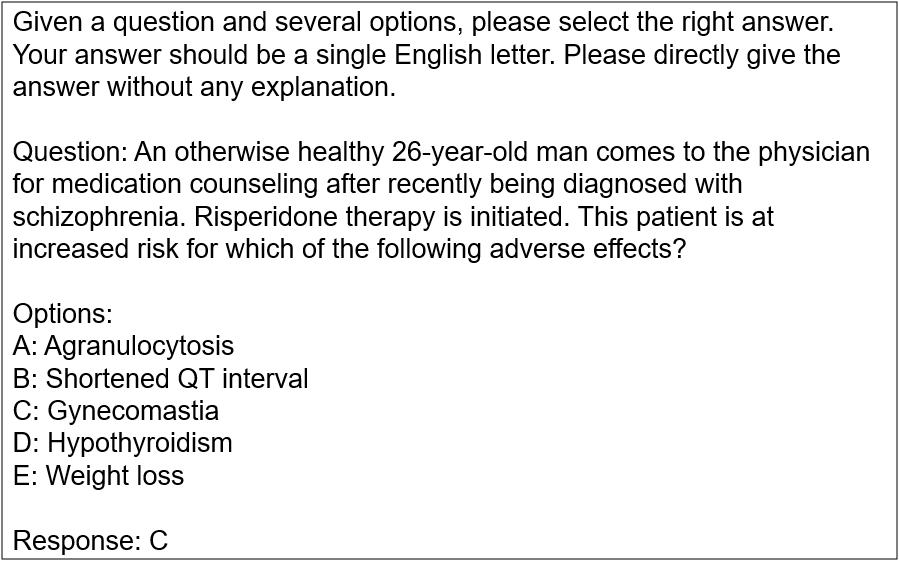
\includegraphics[width=0.45\textwidth]{Figure/Mental_Health_QA.png}
    \caption{Example for Mental Health QA}
    \label{fig: mental health QA}
\end{figure}


   
\subsection{Diagnostic Tasks}
    
\paragraph*{Diagnosis Prediction via Online Text Data.} Leveraging social media for mental health insights is well-established~\cite{chancellor2020methods, culotta2014estimating}. Predicting mental health conditions from online text involves identifying symptoms and correlating them with specific disorders, addressing complex scenarios with multiple diseases.

\textbf{\textit{Data: SMHD}}~\cite{cohan-etal-2018-smhd} is a large dataset of social media posts from users with one or multiple mental health conditions along with matched control users. We employed a classifier~\cite{zhang-etal-2022-symptom} to filter out the sixteen most relevant posts related to mental health diseases from each user's posters. Considering the scale of the post length after filtering and the cost associated with the model's usage, we truly randomly sampled 50 single-label instances for each distinct mental condition, and then truly randomly sampled 50 instances with multiple labels. We provide the model with 16 posters from a user, and the model assesses the potential mental disorders that the user may have based on the content of the posters. 
%\KZ{Is there any annotation efforts on our side? If what we do is just sampling from an existing dataset, why not just take the whole thing? It's a bit weird to random sample 100 or 130 instances from these datasets. Why just 100, why not more?}

\paragraph*{Diagnosis Prediction via Dialogue.} This task employs LLMs and NLP techniques to predict mental health diagnoses from dialogues, inspired by clinical psychology principles~\cite{pacheco-lorenzo2021smart}. Dialogues offer insights into individuals' mental health states, with linguistic cues revealing symptoms and potential diagnoses.

\textbf{\textit{Data: D4}}~\cite{yao-etal-2022-d4} is a Chinese Dialogue Dataset for Depression-Diagnosis-Oriented Chat. It consists of 1,339 multi-turn dialogues with dialogue summary and diagnosis results. Each dialogue is annotated with depression risk and suicide risk scores provided by clinicians, facilitating a 4-way classification for assessing depressive states and suicidal tendencies.
%\MY{say that it enables 4-way classification on depressive state and suicidal tendency. How did you sample the 1/10th? truly random or balanced the categories?} 
Due to the cost of the model's usage, we conducted testing on a truly randomly sampled one-tenth subset of the data. We present the model with a simulated doctor-patient dialogue and task it with scoring the patient's depression risk and suicide risk based on the conversation.

\subsection{Therapeutic Tasks}
    
\paragraph*{Therapeutic Conversations.} This task evaluates LLMs' ability to simulate and understand conversations between psychological counselors and patients in online mental health counseling, a substantiated therapy for mental disorders~\cite{reynolds2013impact}. It has witnessed a surge in popularity, particularly due to the option of anonymous communication~\cite{fu2020effectiveness}.

\textbf{\textit{Data: PsyQA}}~\cite{sun-etal-2021-psyqa}, a Chinese dataset of psychological health support in the form of question and answer pair, is crawled from a Chinese mental health service platform, and contains 22K questions and 56K long and well-structured answers. We truly randomly sampled 100 instances for evaluation. We provide the model with a patient's inquiry and a sequence of strategies, asking the model to respond to the patient like a mental health professional.

\paragraph*{Empathy Capability.} Empathy holds significant weight in the mental health field~\cite{rains2020support}. Assessing LLMs' capacity to exhibit empathy in mental health scenarios is crucial for establishing emotional connections with patients, enhancing the overall patient experience, and improving treatment outcomes.

\textbf{\textit{Data: Esconv}}~\cite{liu-etal-2021-towards}, an Emotional Support Conversation Dataset, which is collected in a help-seeker and supporter mode with crowdworkers, contains 1,300 conversations with 10 topic problems. Each dialogue comes with a label evaluating the mental health counselor's level of empathy. Similarly, we truly randomly selected one-tenth of the data for evaluation. We provide the model with a dialogue in a psychological counseling scenario and instruct it to assess the level of empathy exhibited by the mental health counselor based on the conversation.

\paragraph*{Safety Awareness.} This task evaluates LLMs' proficiency in ensuring safe and responsible therapeutic dialogues in mental health treatment, addressing concerns about dialogue safety in open-domain conversational AI~\cite{rosenthal-etal-2021-solid}.
    
\textit{\textbf{Data: DialogueSafety}}~\cite{qiu2023benchmark} is crawled from an online Chinese text-based counseling platform that provides free counseling services. Each dialog segment comes with a Dialogue Safety Taxonomy label. Due to the model usage costs, we selected all the monologue dialog data from the dataset, totaling 203 instances. We provide the model with a dialogue in a psychological counseling scenario and instruct it to assess the safety categories exhibited by the mental health counselor based on the conversation.

